\documentclass[14pt]{beamer}
% Beamer automatically loads amsmath, amssymb, amsthm, hyperref, graphicx

\usepackage[none]{hyphenat}

\usetheme[progressbar=frametitle]{metropolis}

% THEME
\definecolor{vorange}{HTML}{FF9800}
\definecolor{vgrey}{HTML}{BDBDBD}
\definecolor{vblack}{HTML}{1A1A1A}

\setbeamercolor{progress bar}{fg=vorange, bg=vgrey}
\setbeamercolor{palette primary}{bg=vgrey,fg=white}
 %\setbeamercolor{palette secondary}{bg=vgrey,fg=vorange}
 %\setbeamercolor{palette tertiary}{bg=vgrey,fg=vorange}
 %\setbeamercolor{palette quaternary}{bg=vgrey,fg=vorange}

% FONT
\renewcommand{\familydefault}{\rmdefault}

% BIBLIOGRAPHY
\bibliographystyle{acm}
\setbeamertemplate{bibliography item}{\insertbiblabel}
\setbeamerfont{bibliography item}{size=\tiny}
\setbeamerfont{bibliography entry author}{size=\tiny}
\setbeamerfont{bibliography entry title}{size=\tiny}
\setbeamerfont{bibliography entry location}{size=\tiny}
\setbeamerfont{bibliography entry note}{size=\tiny}

\title{Scraph You Boilerplate}
\subtitle{A Practical Design Pattern for Generic Programming \cite{lammel2003scrap}}
\author{
  Duane~Irvin \\
  \href{mailto:duane@student.chalmers.se}{duane@student.chalmers.se}
}
\institute{
  Room~EG-5215A~---~16~November~13.15\\
  DAT-315~---~The~computer~scientist~in~society\\
  \textsc{Chalmers~University~of~Technology}
}
\date{}

\begin{document}

\begin{frame}\titlepage\end{frame}

\begin{frame}
  \vfill
  \centering\textbf{Apps $>$ Powerpoints}
  \vfill
\end{frame}

%\begin{frame}
  %\textbf{Company Model}
  %\vfill
  %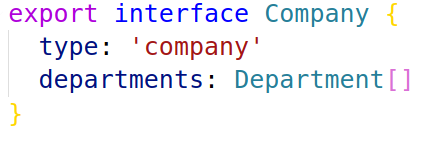
\includegraphics[height=0.272\textheight,width=\textwidth,keepaspectratio]{graphics/interface-company-ts.png}
  %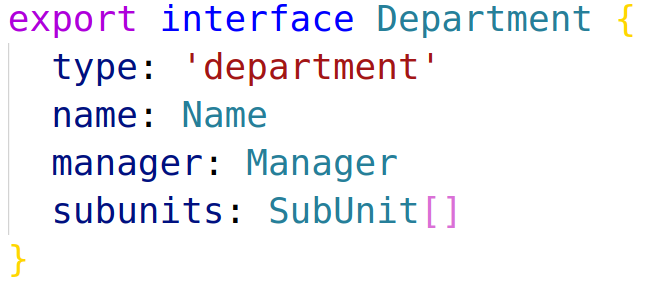
\includegraphics[height=0.4\textheight,width=\textwidth,keepaspectratio]{graphics/interface-department-ts.png}
%\end{frame}

%\begin{frame}
  %\textbf{Employee Model}
  %\vfill
  %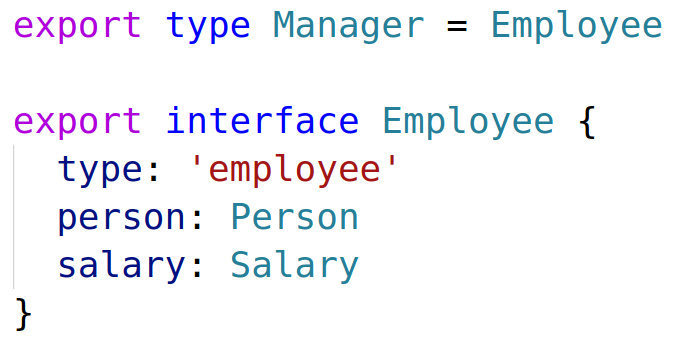
\includegraphics[height=0.4\textheight,width=\textwidth,keepaspectratio]{graphics/interface-employee-ts.png}
  %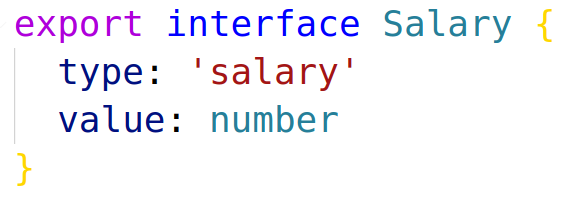
\includegraphics[height=0.264\textheight,width=\textwidth,keepaspectratio]{graphics/interface-salary-ts.png}
%\end{frame}

%\begin{frame}
  %\textbf{Sub unit of department}
  %\vfill
  %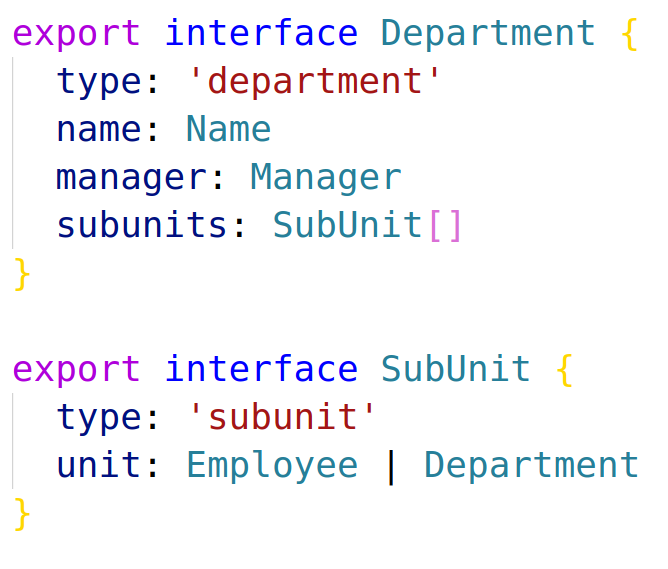
\includegraphics[height=0.8\textheight,width=\textwidth,keepaspectratio]{graphics/interface-subunit-ts.png}
%\end{frame}

\begin{frame}
  \vfill
  \centering\textbf{Let's look at how we'd increase all salaries!}
  \vfill
\end{frame}

\begin{frame}
  \centering\textbf{Increase salary at company}
  \vfill
  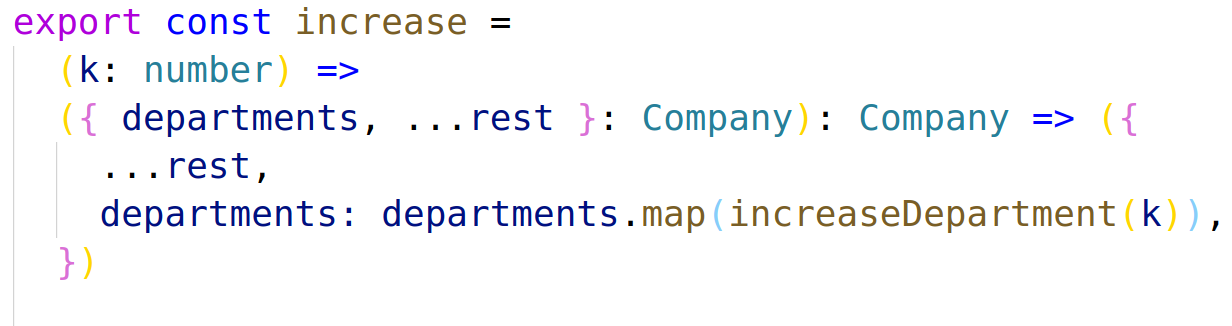
\includegraphics[height=0.9\textheight,width=\textwidth,keepaspectratio]{graphics/increase-naive-step1-ts.png}
\end{frame}

\begin{frame}
  \centering\textbf{Increase salary at each department}
  \vfill
  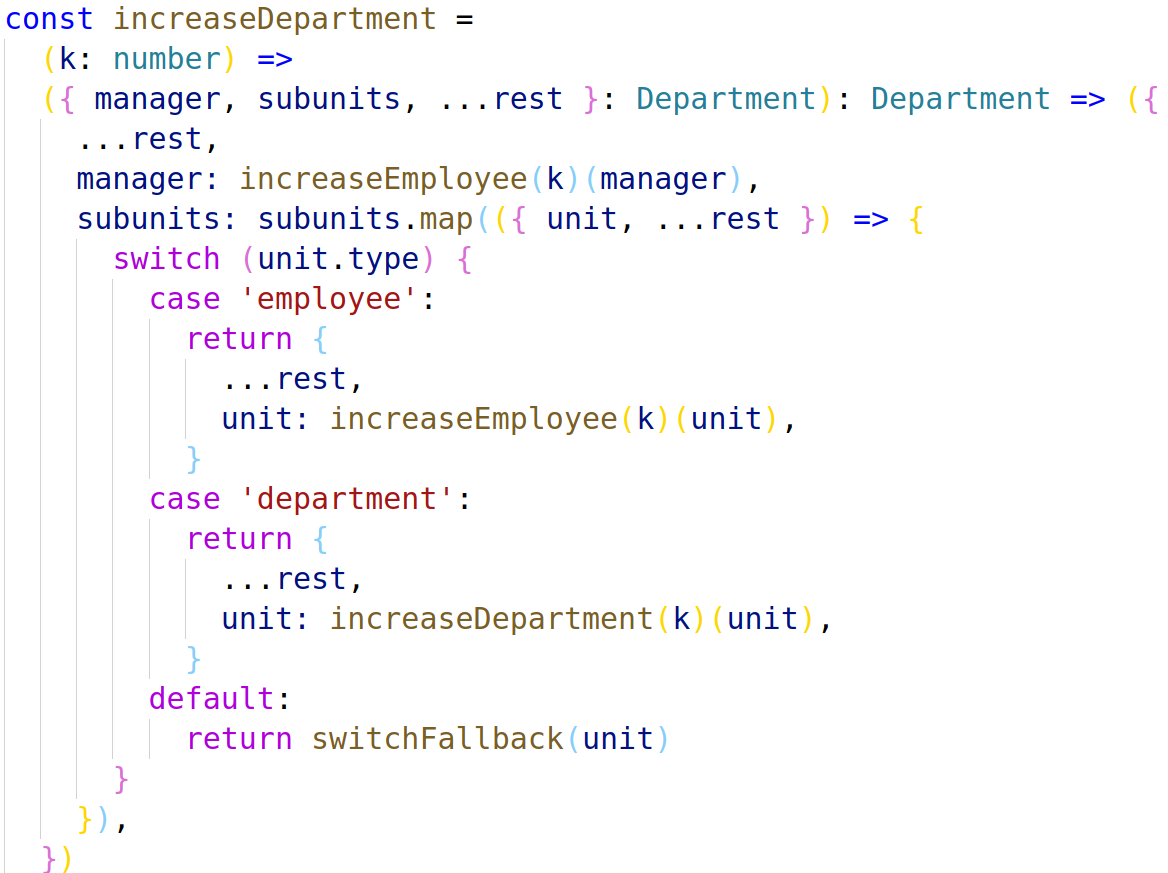
\includegraphics[height=0.8\textheight,width=\textwidth,keepaspectratio]{graphics/increase-naive-step2-ts.png}
\end{frame}

\begin{frame}
  \centering\textbf{Increase salary for each employee}
  \vfill
  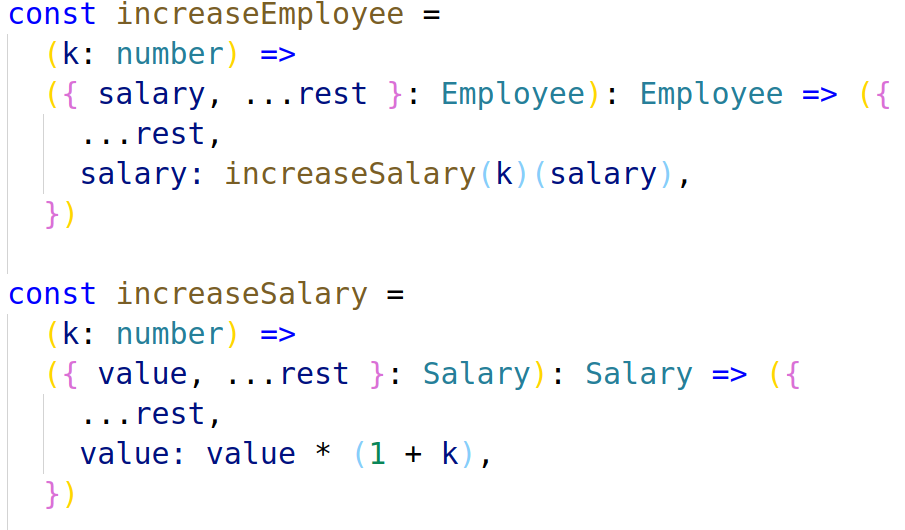
\includegraphics[height=0.9\textheight,width=\textwidth,keepaspectratio]{graphics/increase-naive-step3-ts.png}
\end{frame}

\begin{frame}
  \centering\textbf{That's a lot of code! :(}
  \vfill
  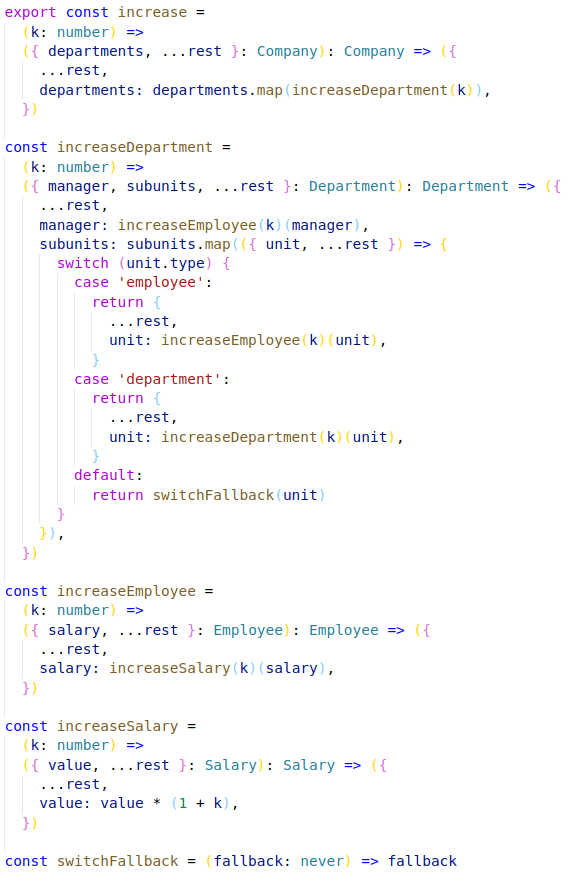
\includegraphics[height=0.8\textheight,width=\textwidth,keepaspectratio]{graphics/increase-naive-ts.png}
\end{frame}

\begin{frame}
  \centering\textbf{What if we could?}
  \vfill
  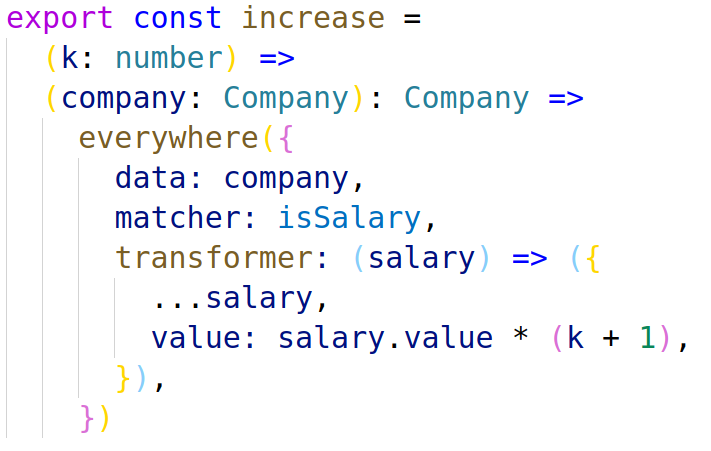
\includegraphics[height=0.8\textheight,width=\textwidth,keepaspectratio]{graphics/increase-ts.png}
\end{frame}

\begin{frame}
  \vfill
  \centering\textbf{Let's look at a different traverse!}
  \vfill
\end{frame}

\begin{frame}
  \begin{columns}
    \begin{column}{.5\textwidth}
      \vspace{1em}
      \centering\textbf{increase Before}
      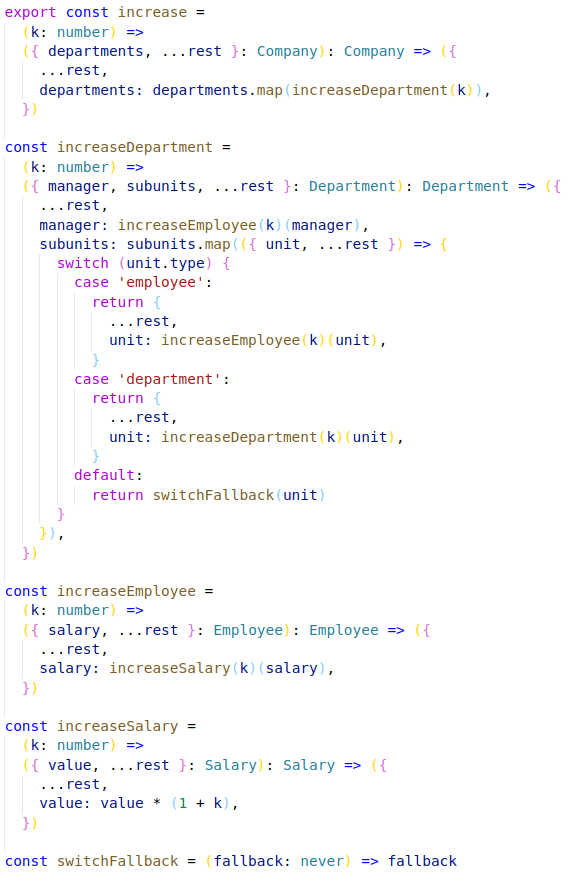
\includegraphics[height=0.7\textheight,width=\textwidth,keepaspectratio]{graphics/increase-naive-ts.png}
    \end{column}
    \begin{column}{.5\textwidth}
      \vspace{1em}
      \centering\textbf{increase After}
      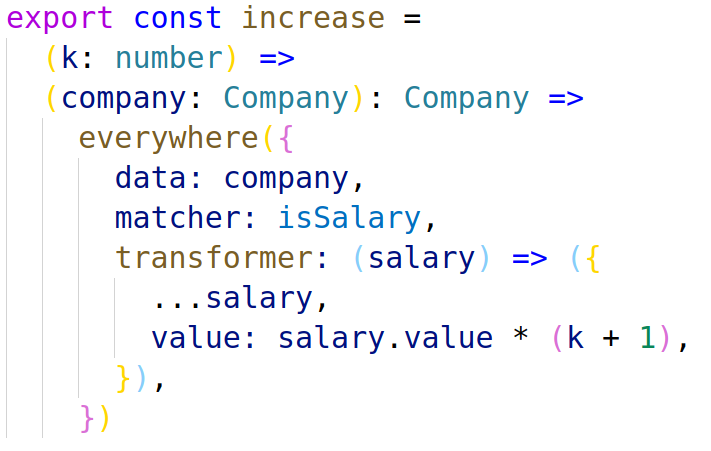
\includegraphics[height=0.7\textheight,width=\textwidth,keepaspectratio]{graphics/increase-ts.png}
    \end{column}
  \end{columns}
\end{frame}

\begin{frame}
  \begin{columns}
    \begin{column}{.5\textwidth}
      \vspace{1em}
      \centering\textbf{bill Before}
      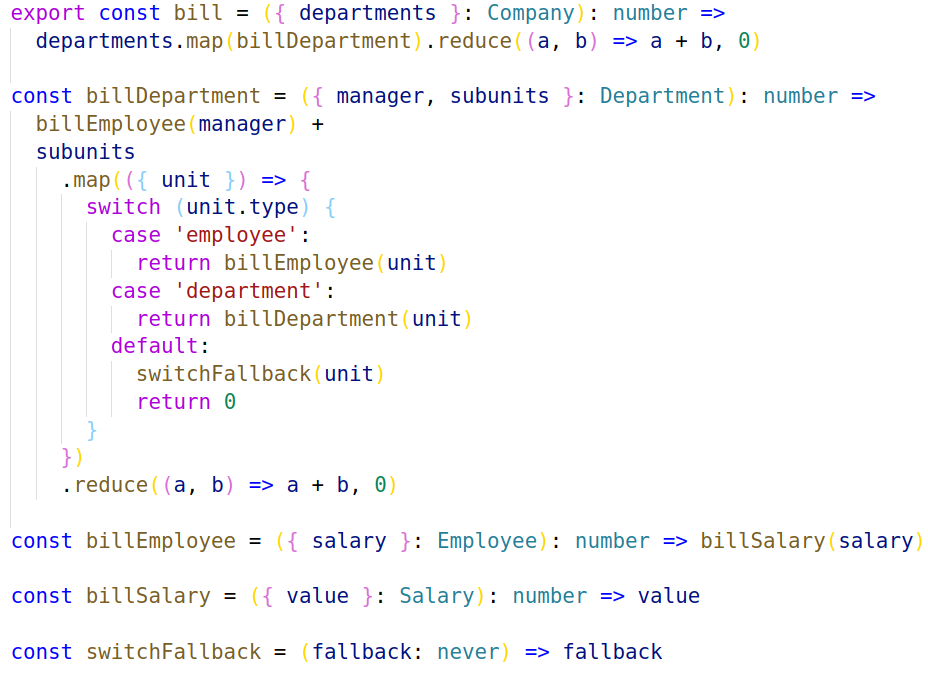
\includegraphics[height=0.7\textheight,width=\textwidth,keepaspectratio]{graphics/bill-naive-ts.png}
    \end{column}
    \begin{column}{.5\textwidth}
      \vspace{1em}
      \centering\textbf{bill After}
      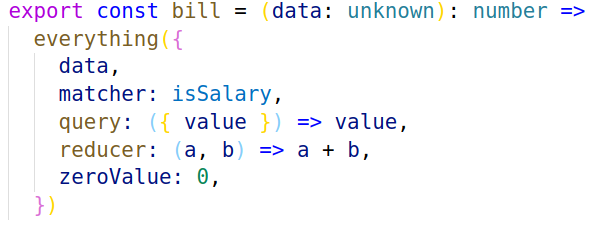
\includegraphics[height=0.7\textheight,width=\textwidth,keepaspectratio]{graphics/bill-ts.png}
    \end{column}
  \end{columns}
\end{frame}

\begin{frame}
  \centering\textbf{Haskell Before}
  \vfill
  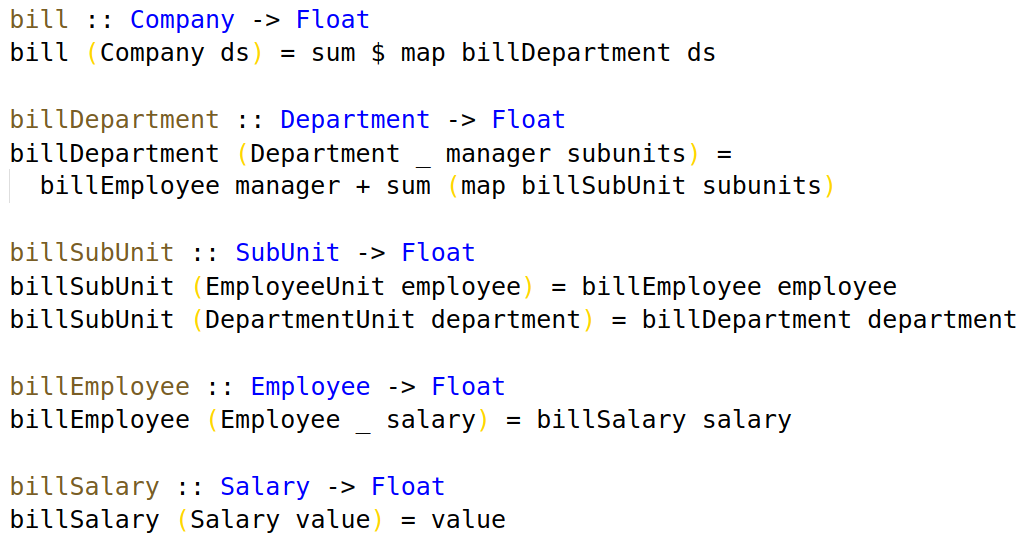
\includegraphics[height=0.8\textheight,width=\textwidth,keepaspectratio]{graphics/bill-naive-hs.png}
  \vfill
\end{frame}

\begin{frame}
  \centering\textbf{Haskell After}
  \vfill
  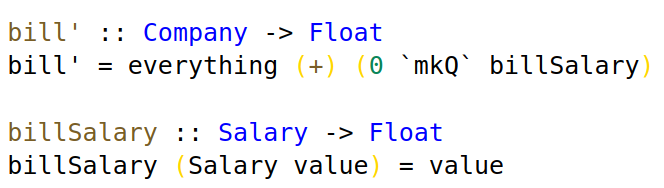
\includegraphics[height=0.8\textheight,width=\textwidth,keepaspectratio]{graphics/bill-hs.png}
  \vfill
\end{frame}

\begin{frame}
  \vfill
  \centering\textbf{Key idea}
  \vfill
  \centering
  Rethink how we traverse data
  \vfill
  $\Downarrow$
  \vfill
  Pure boilerplate can separated and generated
  \vfill
\end{frame}

\begin{frame}
  \centering\textbf{Prior related work}
  \vfill
  A new approach to generic functional programming. Hinze, R., 2000 \cite{hinze2000new}
  \vfill
  \small{But poly-typic programming is too strict to be useful}
  \vfill
\end{frame}

\begin{frame}
  \centering\textbf{Derivative work}
  \vfill
  Go beyond \texttt{show}, \texttt{map} and \texttt{reduce}:\\
  \vfill
  ``Scrap Your Boilerplate'' Revolutions. Hinze, R., and L\"{o}h, 2006 \cite{hinze2006scrap}
  \vfill
\end{frame}

\begin{frame}[fragile]\frametitle{References}
  \bibliography{include/backmatter/Bibliography}
  \small{Source code: \href{https://github.com/irvin93d/scrap-your-boilerplate}{github.com/irvin93d/scrap-your-boilerplate}}
\end{frame}

\end{document}
